% !TeX root = ../main.tex
\chapter{系統實驗與結果討論}

    本章將說明本論文研究所提出之系統的實作與實驗。
首先說明系統各角色之實作細節,並於接續章節說明實驗與結果討論。

\section{系統實作}

    本章節將說明本論文研究所提出的協定與硬體之實作,包含「會談終端」、「解封伺服器」
與供會談主持者用於與解封伺服器通訊的「行動應用程式」。

\subsection{會談終端}\label{subsec:impl-mbox}

    會談終端包含多個組件,其概念驗證實作硬體組成如圖 \ref{fig:mbox}。

\begin{figure}[H]
    \centering
    \includegraphics[width=1.0\textwidth]{mbox}
    \caption{會談終端概念驗證實作}\label{fig:mbox}
\end{figure}


\paragraph{超音波麥克風干擾器}

    如圖 \ref{fig:mbox} \nameref{fig:mbox}中左下紫色實線多邊形方框所示。
此超音波麥克風干擾器為參考 Yuxin Chen,  Huiying Li 等人的實作\cite{chen2020wearable}。
包含一 Arduino Micro 用於產生於$24k\sim26k$之間的偽隨機數與控制周邊裝置。
包含一波形產生器 AD9833,透過SPI與Arduino Micro溝通取得偽隨機數,產生介於$24khz\sim26khz$之間正弦波。
包含一數位放大器 HW-104,用於放大訊號產生器產生的訊號以驅動超音波發射器。
包含一超音波發射器,產生介於$24khz\sim26khz$之間的超音波。
此超音波麥克風干擾器於系統時脈$16Mhz$的單晶片控制器中,每 $2ms$ 產生新的偽隨機數,使其生成干擾超音波。

\paragraph{錄音麥克風}

    如圖 \ref{fig:mbox} \nameref{fig:mbox}中左上黃色實線圓框所示。
包含一USB數位駐極電容式麥克風 Saramonic LavMicro U3A。
用於錄製受超音波麥克風干擾器干擾的會談對話聲音記錄 (\DEFrecJ),
與產生純超音波麥克風干擾器於麥克風的響應輸出(純噪音)之聲音記錄 (\DEFrecN)。

\paragraph{物理控制介面}

    如圖 \ref{fig:mbox} \nameref{fig:mbox}中左上紅色虛線圓框所示。
本系統實作以按鈕為例,提供會談參與者操作與會談終端互動,獲得外部觸發事件,`
用於創建、開始與結束會談。

\paragraph{人機互動介面}

    如圖 \ref{fig:mbox} \nameref{fig:mbox}中右上紅色點虛線方框所示。
本系統實作以電子紙為例,用於傳遞會談的元資料與系統狀態提示給會談主持者與提示系統狀態給會談參與者。
會談主持者透過掃描電子紙螢幕上的 QRCode 接收來自會談終端傳遞的會談的元資料,如圖 \ref{fig:epaper}。
本系統實作按鈕含有一指示燈兼作人機互動介面,於談開始/結束錄音提示系統狀態,如圖 \ref{fig:btn}。

\begin{figure}[H]
    \centering
    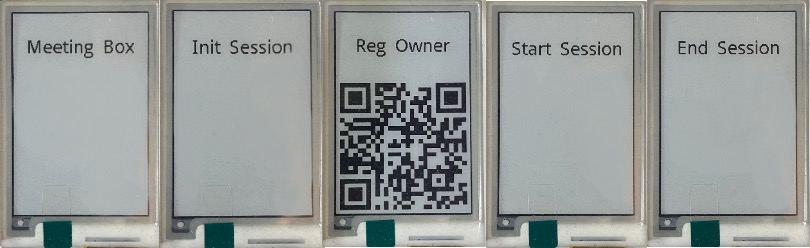
\includegraphics[width=1.0\textwidth]{epaper}
    \caption{電子紙於會談各階段之狀態顯示}\label{fig:epaper}
\end{figure}

\begin{figure}[H]
    \centering
    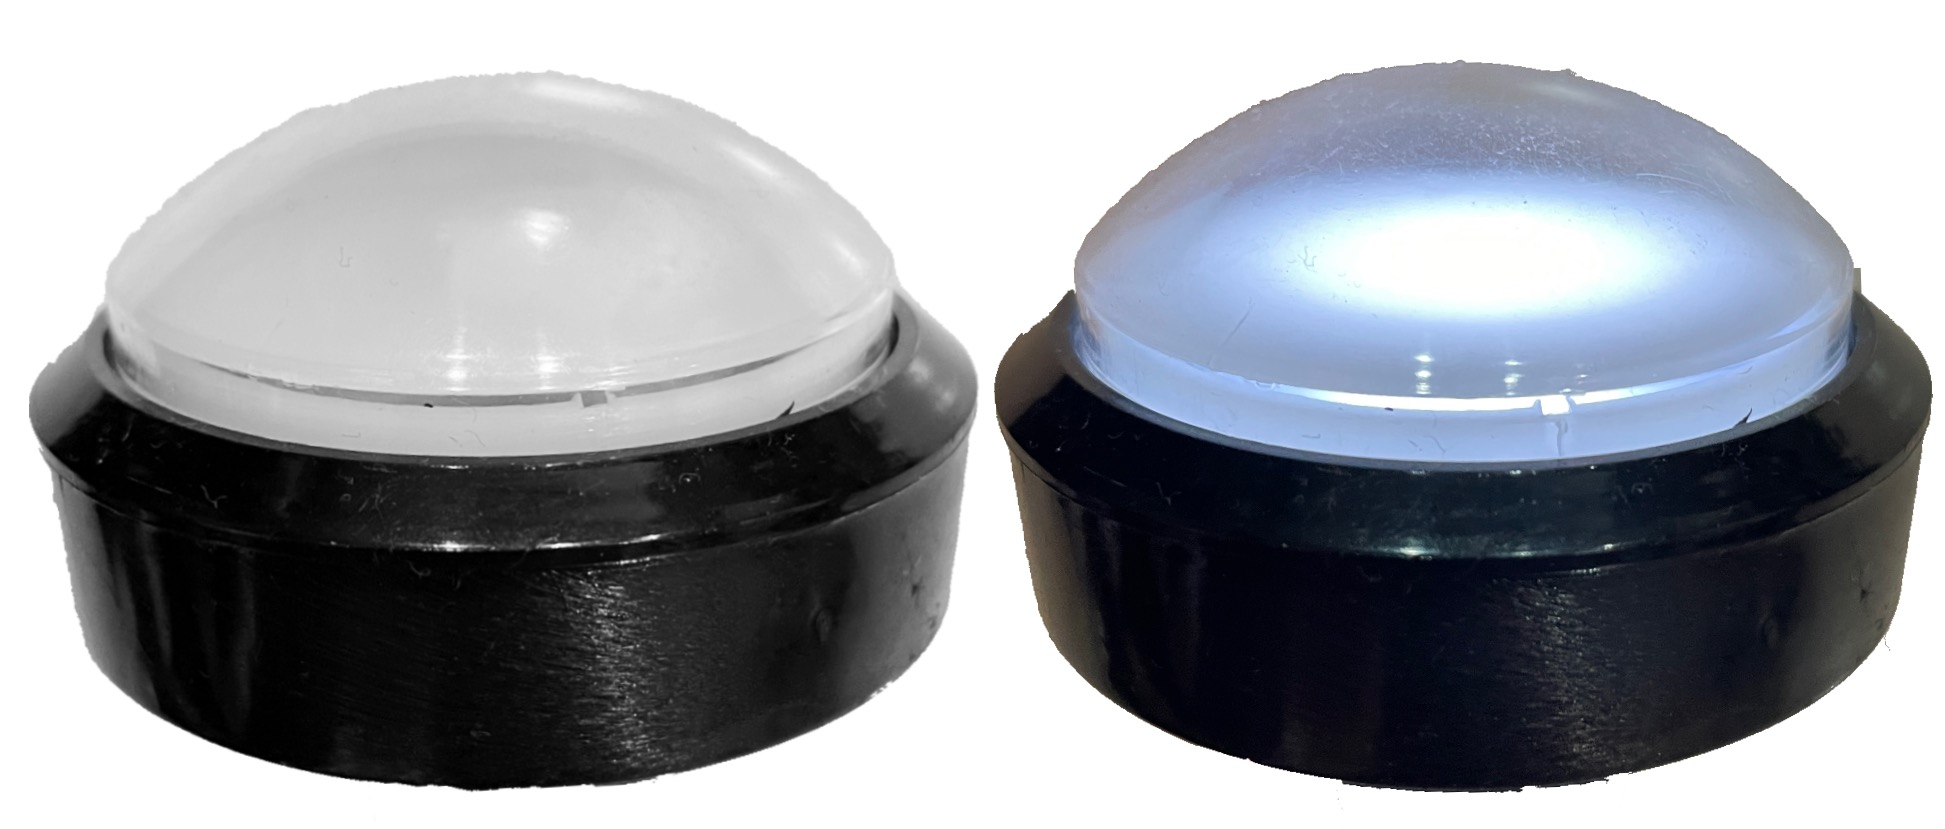
\includegraphics[width=0.5\textwidth]{btn}
    \caption{按鈕於會談開始/結束錄音之狀態指示燈}\label{fig:btn}
\end{figure}

\paragraph{運算控制核心與網路介面}

    如圖 \ref{fig:mbox} \nameref{fig:mbox}中右下綠色點線方框所示。
本系統實作以 Raspberry Pi 4B 為例,包含一 Geekworm X728 電池模組用於供電。
邏輯控制核心使用 Python 實作,控制周邊裝置包含人機互動介面、物理控制介面、超音波麥克風干擾器與錄音麥克風,
並網路介面與解封伺服器溝通。透過 GPIO 接收來自物理控制介面介面的外部觸發事件;透過 SPI 介面控制人機互動介面;
透過 GPIO 控制一外部 MOSFET 開啟關閉超音波干擾器;透過 fork/exec 呼叫 arecord 透過麥克風進行錄音;



\subsection{解封伺服器}

    本研究所設計之系統中解封伺服器的服務介面 RESTful\cite{fielding2000architectural} API 組成,
包含數個 API 端點,使用 Golang 搭配 Gin 網頁框架實作。
系統後端組件包含一資料庫 PostgreSQL 13 作為資料關聯綁定以及儲存的媒介;
包含 Docker 容器化執行引擎,用於封裝主動式噪音消除的 Python3 執行環境;
各 API 端點說明如下。

\begin{enumerate}
    \item \texttt{POST},~ \texttt{/meeting/}

        此 API 端點實作章節 \ref{sec:protocol} \nameref{sec:protocol}中,
    \nameref{subsec:protocol-init-create} 的 $M_{1}$ 、 $M_{2}$。
    當 API 端點收到請求後,會執行 \DEFfuncIDgen{} 與 \DEFfuncKgen{},
    分別產生此次會談的唯一識別碼 \DEFsessionID,與此次會談的解封金鑰 \DEFunsealKey。

        其中 \DEFfuncIDgen{} 為唯一識別碼產生函數,其產生須滿足唯一性、隨機性、不可預測性,
    本研究實作以 UUID \cite{rfc4122} 為例。
    \DEFfuncKgen{} 為對稱式加密演算法的金鑰產生函數,
    本研究實作以 AES CFB 模式 \cite{117146}\cite{9171} 為例。

    \item \texttt{POST},~ \texttt{/meeting/:id/owner}

        此 API 端點實作章節 \ref{sec:protocol} \nameref{sec:protocol}中,
    \nameref{subsec:protocol-init-reg} 的 $M_{3}^{i}$ 、 $M_{4}^{i}$。
    當 API 端點收到請求後,會執行 \DEFfuncPKgen{} 與 \DEFfuncIDgen{},
    分別產生一組屬於會談主持者 \DEFowner 的公開私密金鑰對 $($\DEFpublicKey$,~$ \DEFprivateKey$)$,
    與此會談主持者 \DEFowner 的唯一識別碼 \DEFownerID。

        其中會談主持者的唯一識別碼 \DEFownerID,其產生須滿足唯一性、隨機性、不可預測性,
    本研究實作以 UUID \cite{rfc4122} 為例。
    \DEFfuncPKgen{} 為非對稱加密演算法的公開私密金鑰對產生函數,
    本研究實作以 RSA PKCS\#1 \cite{rfc8017} 為例。
    路由變數 \texttt{:id} 為此次會談的唯一識別碼 \DEFsessionID。

    \item \texttt{POST},~ \texttt{/meeting/:id/end}

        此 API 端點實作章節 \ref{sec:protocol} \nameref{sec:protocol}中,
    \nameref{subsec:protocol-sessioning} 的 $M_{1}$ 、 $M_{2}$。
    當 API 端點收到請求後,主持者註冊人數 \DEFowreg 是否為一或多人,
    可能執行非對稱式金鑰演算法加密函數 \DEFfuncEncPK{} 或金鑰分割函數 \DEFfuncSSS{}。

        其中 \DEFfuncEncPK{} 為非對稱式金鑰演算法加密函數,本研究實作以 RSA PKCS\#1 \cite{rfc8017} 為例。
    \DEFfuncSSS{} 為金鑰分割函數,
    本研究實作以 Shamir's Secret Sharing \cite{shamir1979share} 於 $GF(2^8)$ 的實作 \cite{117146} 為例。
    路由變數 \texttt{:id} 為此次會談的唯一識別碼 \DEFsessionID。

    \item \texttt{POST},~ \texttt{/unseal/:id/rec/:kind}

        此 API 端點實作根據路由中變數 \texttt{:kind} 可能為章節 \ref{sec:protocol} \nameref{sec:protocol}中,
    \nameref{subsec:protocol-init-create} 的 $M_{3}$ 、 $M_{4}$,
    或章節 \ref{sec:protocol} \nameref{sec:protocol}中,
    \nameref{subsec:protocol-sessioning} 的 $M_{3}$ 、 $M_{4}$。
    其功能皆為上傳錄音,透過判斷路由中變數 \texttt{:kind} 得知上傳的是何種錄音,
    執行關聯綁定屬於此次會談的唯一識別碼 \DEFsessionID。
    路由變數 \texttt{:id} 為此次會談的唯一識別碼 \DEFsessionID。

    \item \texttt{GET},~ \texttt{/unseal/:meetingid/:ownerid}

        此 API 端點實作章節 \ref{sec:protocol} \nameref{sec:protocol}中,
    \nameref{subsec:protocol-unseal-auth} 的 $M_{1}^{i}$ 、 $M_{2}^{i}$。
    路由變數 \texttt{:meetingid} 為此次會談的唯一識別碼 \DEFsessionID。
    路由變數 \texttt{:ownerid} 為會談主持者唯一識別碼 \DEFownerID。

    \item \texttt{PUT},~ \texttt{/unseal/:meetingid/:ownerid}

        此 API 端點實作章節 \ref{sec:protocol} \nameref{sec:protocol}中,
    \nameref{subsec:protocol-unseal-auth} 的 $M_{3}^{i}$ 、 $M_{4}^{i}$。
    會談主持者的私密金鑰 \DEFprivateKey,透過非對稱式加密演算法之解密函數 \DEFfuncDecSK{},
    將受加密保護的授權金鑰 \DEFakEnc 解密,接著使用同一會談主持者的私密金鑰 \DEFprivateKey,
    透過數位簽章演算法簽之簽名函數 \DEFfuncSignSK{}。
    解封伺服器 \DEFserver 使用會談主持者的公開金鑰 \DEFpublicKey,
    透過數位簽章演算法簽之驗證函數 \DEFfuncVerfPK{},驗證解密後的授權金鑰與其簽名。

        其中 \DEFfuncDecSK{} 為非對稱式加密演算法之解密函數;\DEFfuncSignSK{} 為數位簽章演算法簽之簽名函數;
    \DEFfuncVerfPK{} 為過數位簽章演算法簽之驗證函數;本研究實作以 RSA PKCS\#1 \cite{rfc8017} 為例。
    路由變數 \texttt{:meetingid} 為此次會談的唯一識別碼 \DEFsessionID。
    路由變數 \texttt{:ownerid} 為會談主持者唯一識別碼 \DEFownerID。

    \item \texttt{GET},~ \texttt{/unseal/:meetingid/access}

        此 API 端點實作章節 \ref{sec:protocol} \nameref{sec:protocol}中,
    \nameref{subsec:protocol-unseal-access} 的 $M_{1}$ 、 $M_{2}$。
    當 API 端點收到請求後,主持者註冊人數 \DEFowreg 是否為一或多人,
    可能執行對稱式加密演算法之解密函數 \DEFfuncDecEK{} 或金鑰分割演算法合併函數 \DEFfuncSSC{}。
    接著透過聲音樣本的離散時間誤差推估函數 \DEFfuncEstm{},得到兩聲音樣本的離散時間對齊誤差值 \DEFshift。
    再透過自適應噪音消除 \DEFfuncAnc{},還原獲得有效的會談聲音記錄 \DEFrecREV。

        其中 \DEFfuncDecEK{} 對稱式加密演算法之解密函數,
    為本研究實作以 AES CFB 模式 \cite{117146}\cite{9171} 為例。
    \DEFfuncSSC{} 為金鑰分割演算法合併函數。
    本研究實作以 Shamir's Secret Sharing \cite{shamir1979share} 於 $GF(2^8)$ 的實作 \cite{117146} 為例。
    路由變數 \texttt{:meetingid} 為此次會談的唯一識別碼 \DEFsessionID。

        其中 \DEFfuncEstm{} 離散時間誤差推估函數,透過 \texttt{goroutine} 於背景中執行。
    此為 Golang 的輕量執行緒,此函式呼叫為非阻塞式呼叫。
    \DEFfuncAnc{} 為自適應噪音消除函數,
    本研究實作以引用 M Cejnek 的自適應訊號處理開源函式庫 \cite{cejnek2017padasip} 為例。
    透過 Docker 於容器環境 \texttt{jupyter/scipy-notebook} 中執行。
    此呼叫利用 \texttt{goroutine} 於背景中執行,為非阻塞式呼叫。
\end{enumerate}


\subsection{行動應用程式}

    會談主持者持有智慧型裝置,且透過行動應用程式(mobile application)與會談終端互動,獲取會談終端上的資訊。
並有能力於各階端包含會談初始化、會談進行中、談結束後,與解封伺服器進行通訊。
本研究實作以單頁應用(Single-page Application, SPA)為例。

    談主持者透過會談終端 \DEFmeetingbox 上的人機互動介面,
取得此次會談的元資料與封伺服器的資源位置 URI (Uniform Resource Identifier),
本研究實作以描電子紙螢幕上搭配顯示 QRCode 為例。
會談主持者透過掃描會談終端的電子紙螢幕上顯示的 QRCode 取得資源位置,接著向解封伺服器 \DEFserver 請求註冊,
註冊成功則成為此次會談的會談主持者,並取得代表會談主持者身份的私密金鑰。
如圖 \ref{fig:app-1} \nameref{fig:app-1},
圖 \ref{fig:app-1} 左圖為掃描 QRCode 使用者介面,右圖為的會談主持者註冊使用者介面。

\begin{figure}[H]
    \centering
    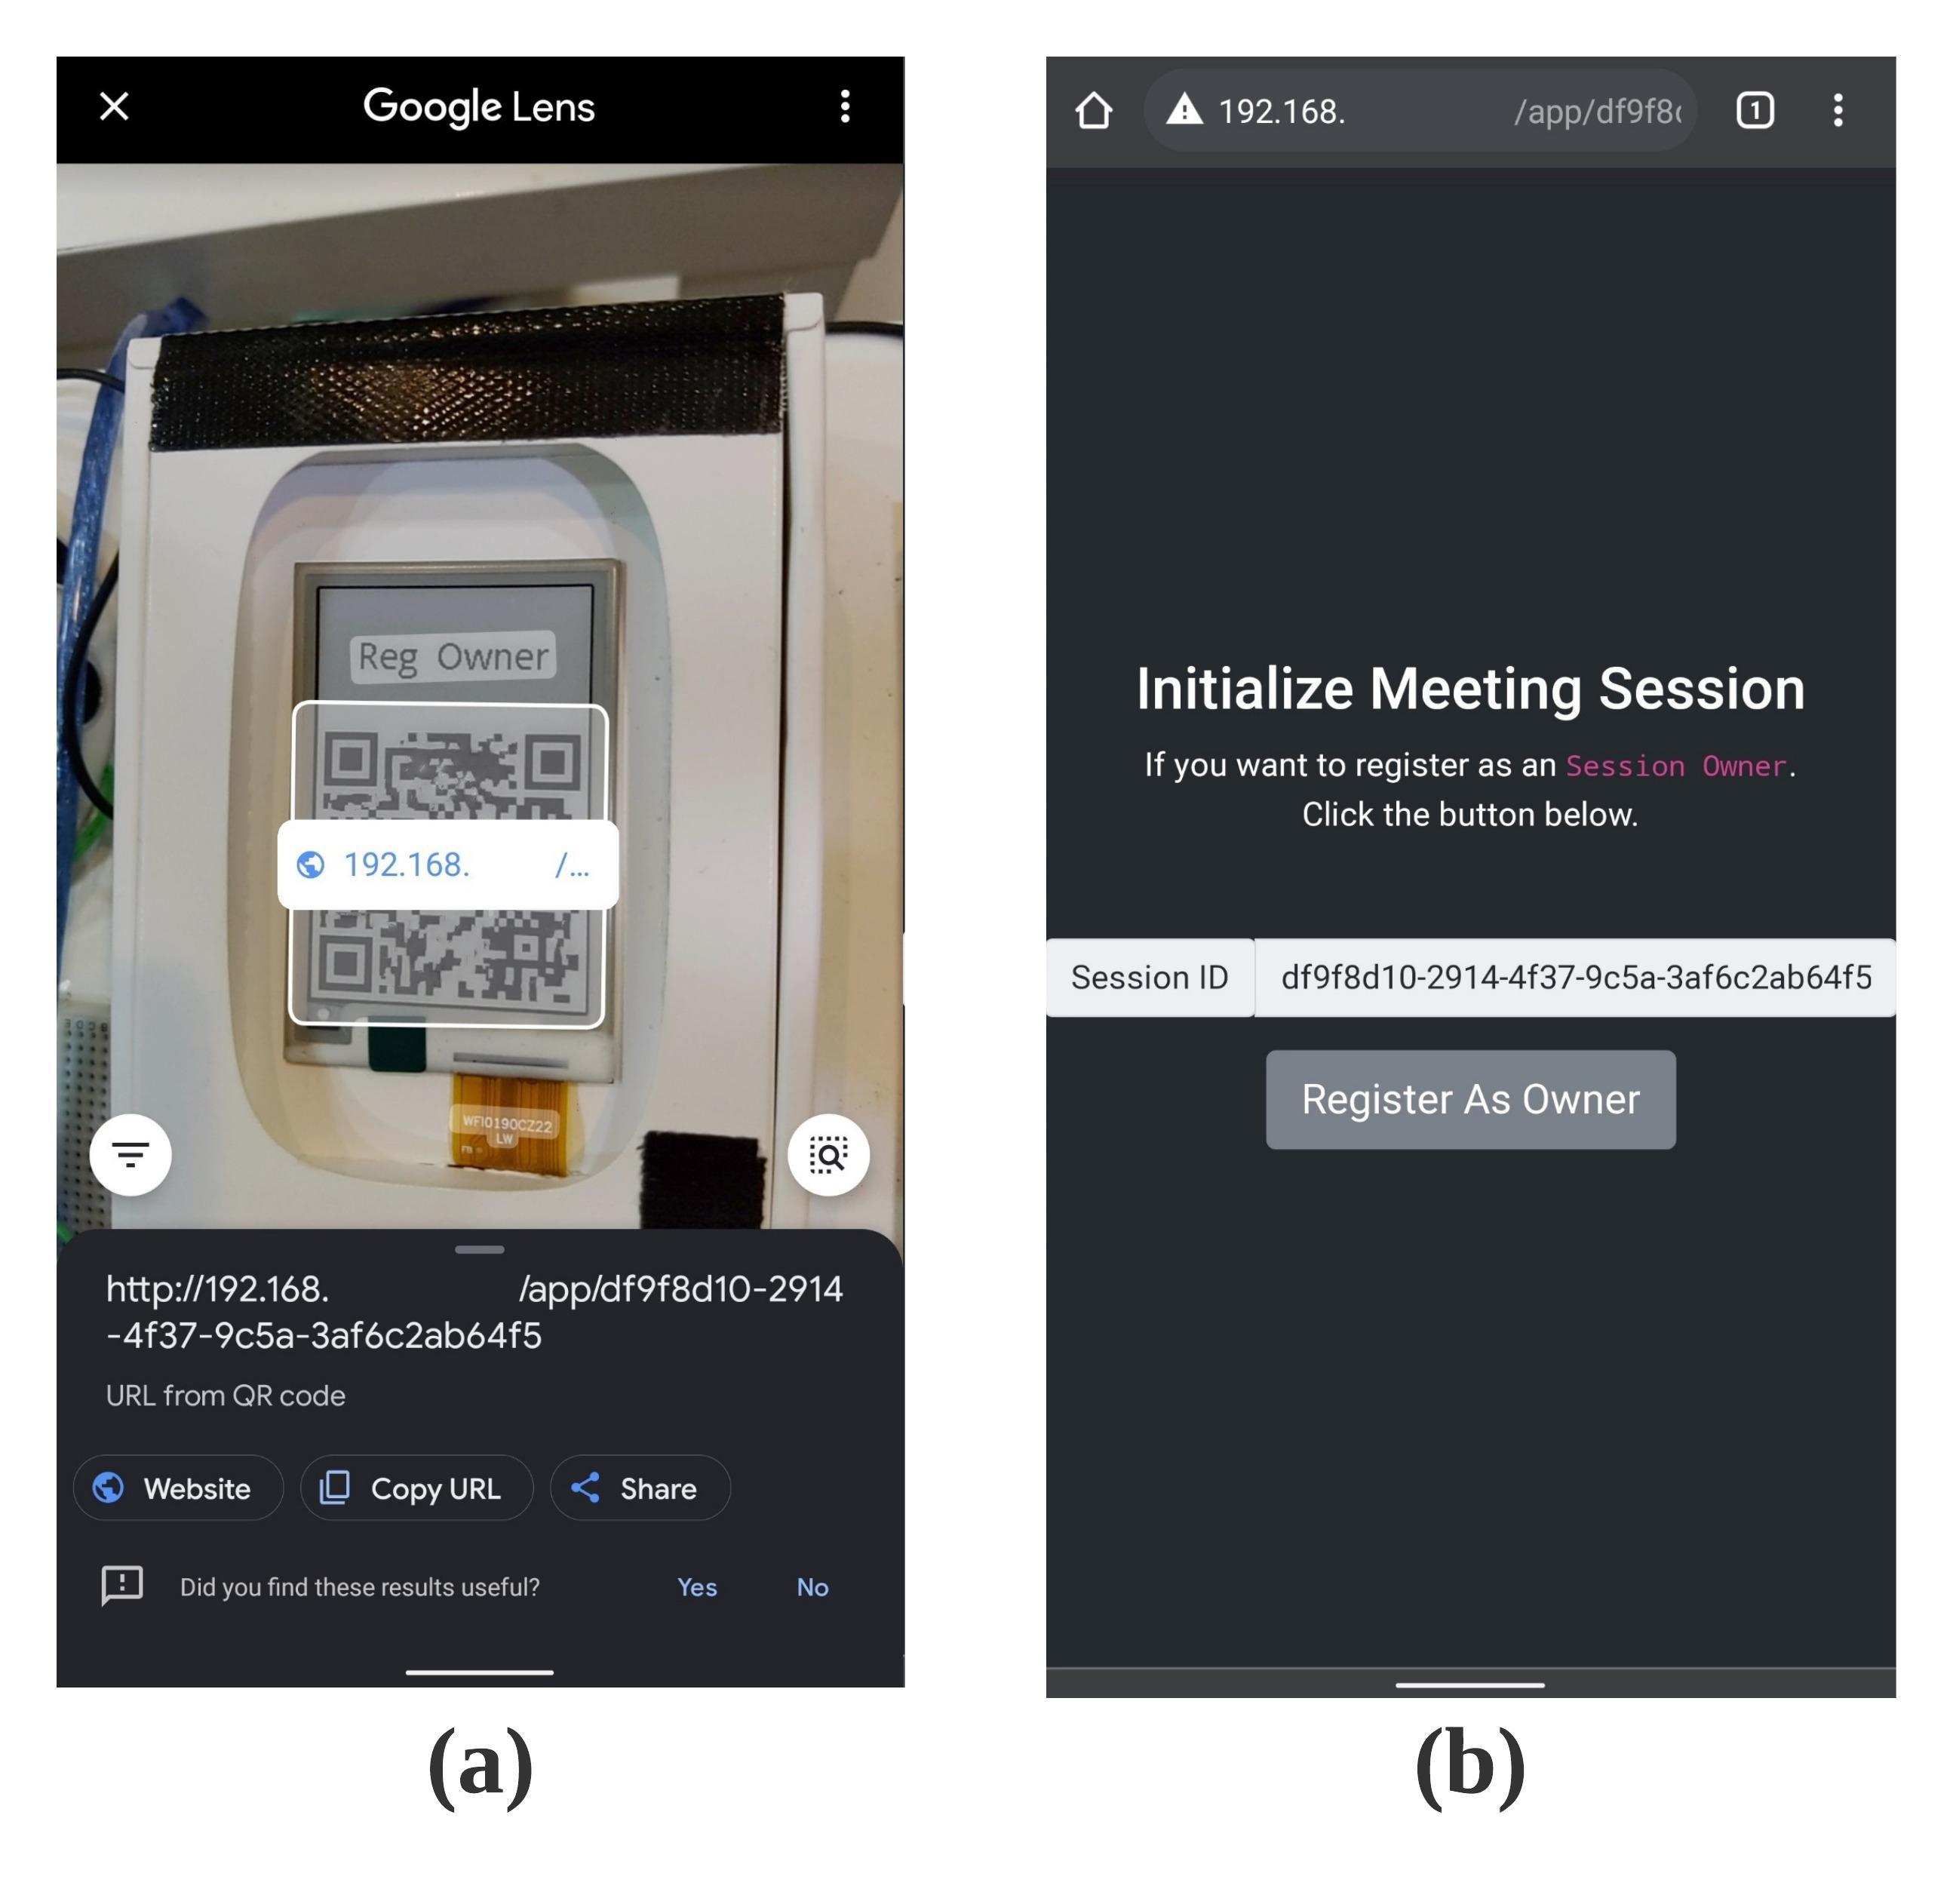
\includegraphics[width=0.5\textwidth]{app-1}
    \caption{行動應用程式會談初始化使用者介面}\label{fig:app-1}
\end{figure}

    在會談對話結束後,會談主持者欲取得當時會談的有效聲音紀錄,須先授權解封伺服器 \DEFserver。
此時會談主持者向解封伺服器 \DEFserver 傳送授權解封聲音會談記錄請求。
如圖 \ref{fig:app-2} \nameref{fig:app-2}(左一)。

    解封伺服器 \DEFserver 收到授權解封聲音會談記錄請求後,即依據會談主持者的唯一識別碼 \DEFownerID,
回覆屬於會談主持者的受加密保護的授權金鑰 \DEFakEnc 請會談主持者簽署授權。
如圖 \ref{fig:app-2} \nameref{fig:app-2}的(中)。
並透過代表會談主持者身份的私密金鑰,證明會談主持者的身份與授權解封伺服器。
會談主持者的私密金鑰 \DEFprivateKey,透過非對稱式加密演算法之解密函數 \DEFfuncDecSK{},
將受加密保護的授權金鑰 \DEFakEnc 解密,接著使用同一會談主持者的私密金鑰 \DEFprivateKey,
透過數位簽章演算法簽之簽名函數 \DEFfuncSignSK{}。
如圖 \ref{fig:app-2} \nameref{fig:app-2}(右一)。

\begin{figure}[H]
    \centering
    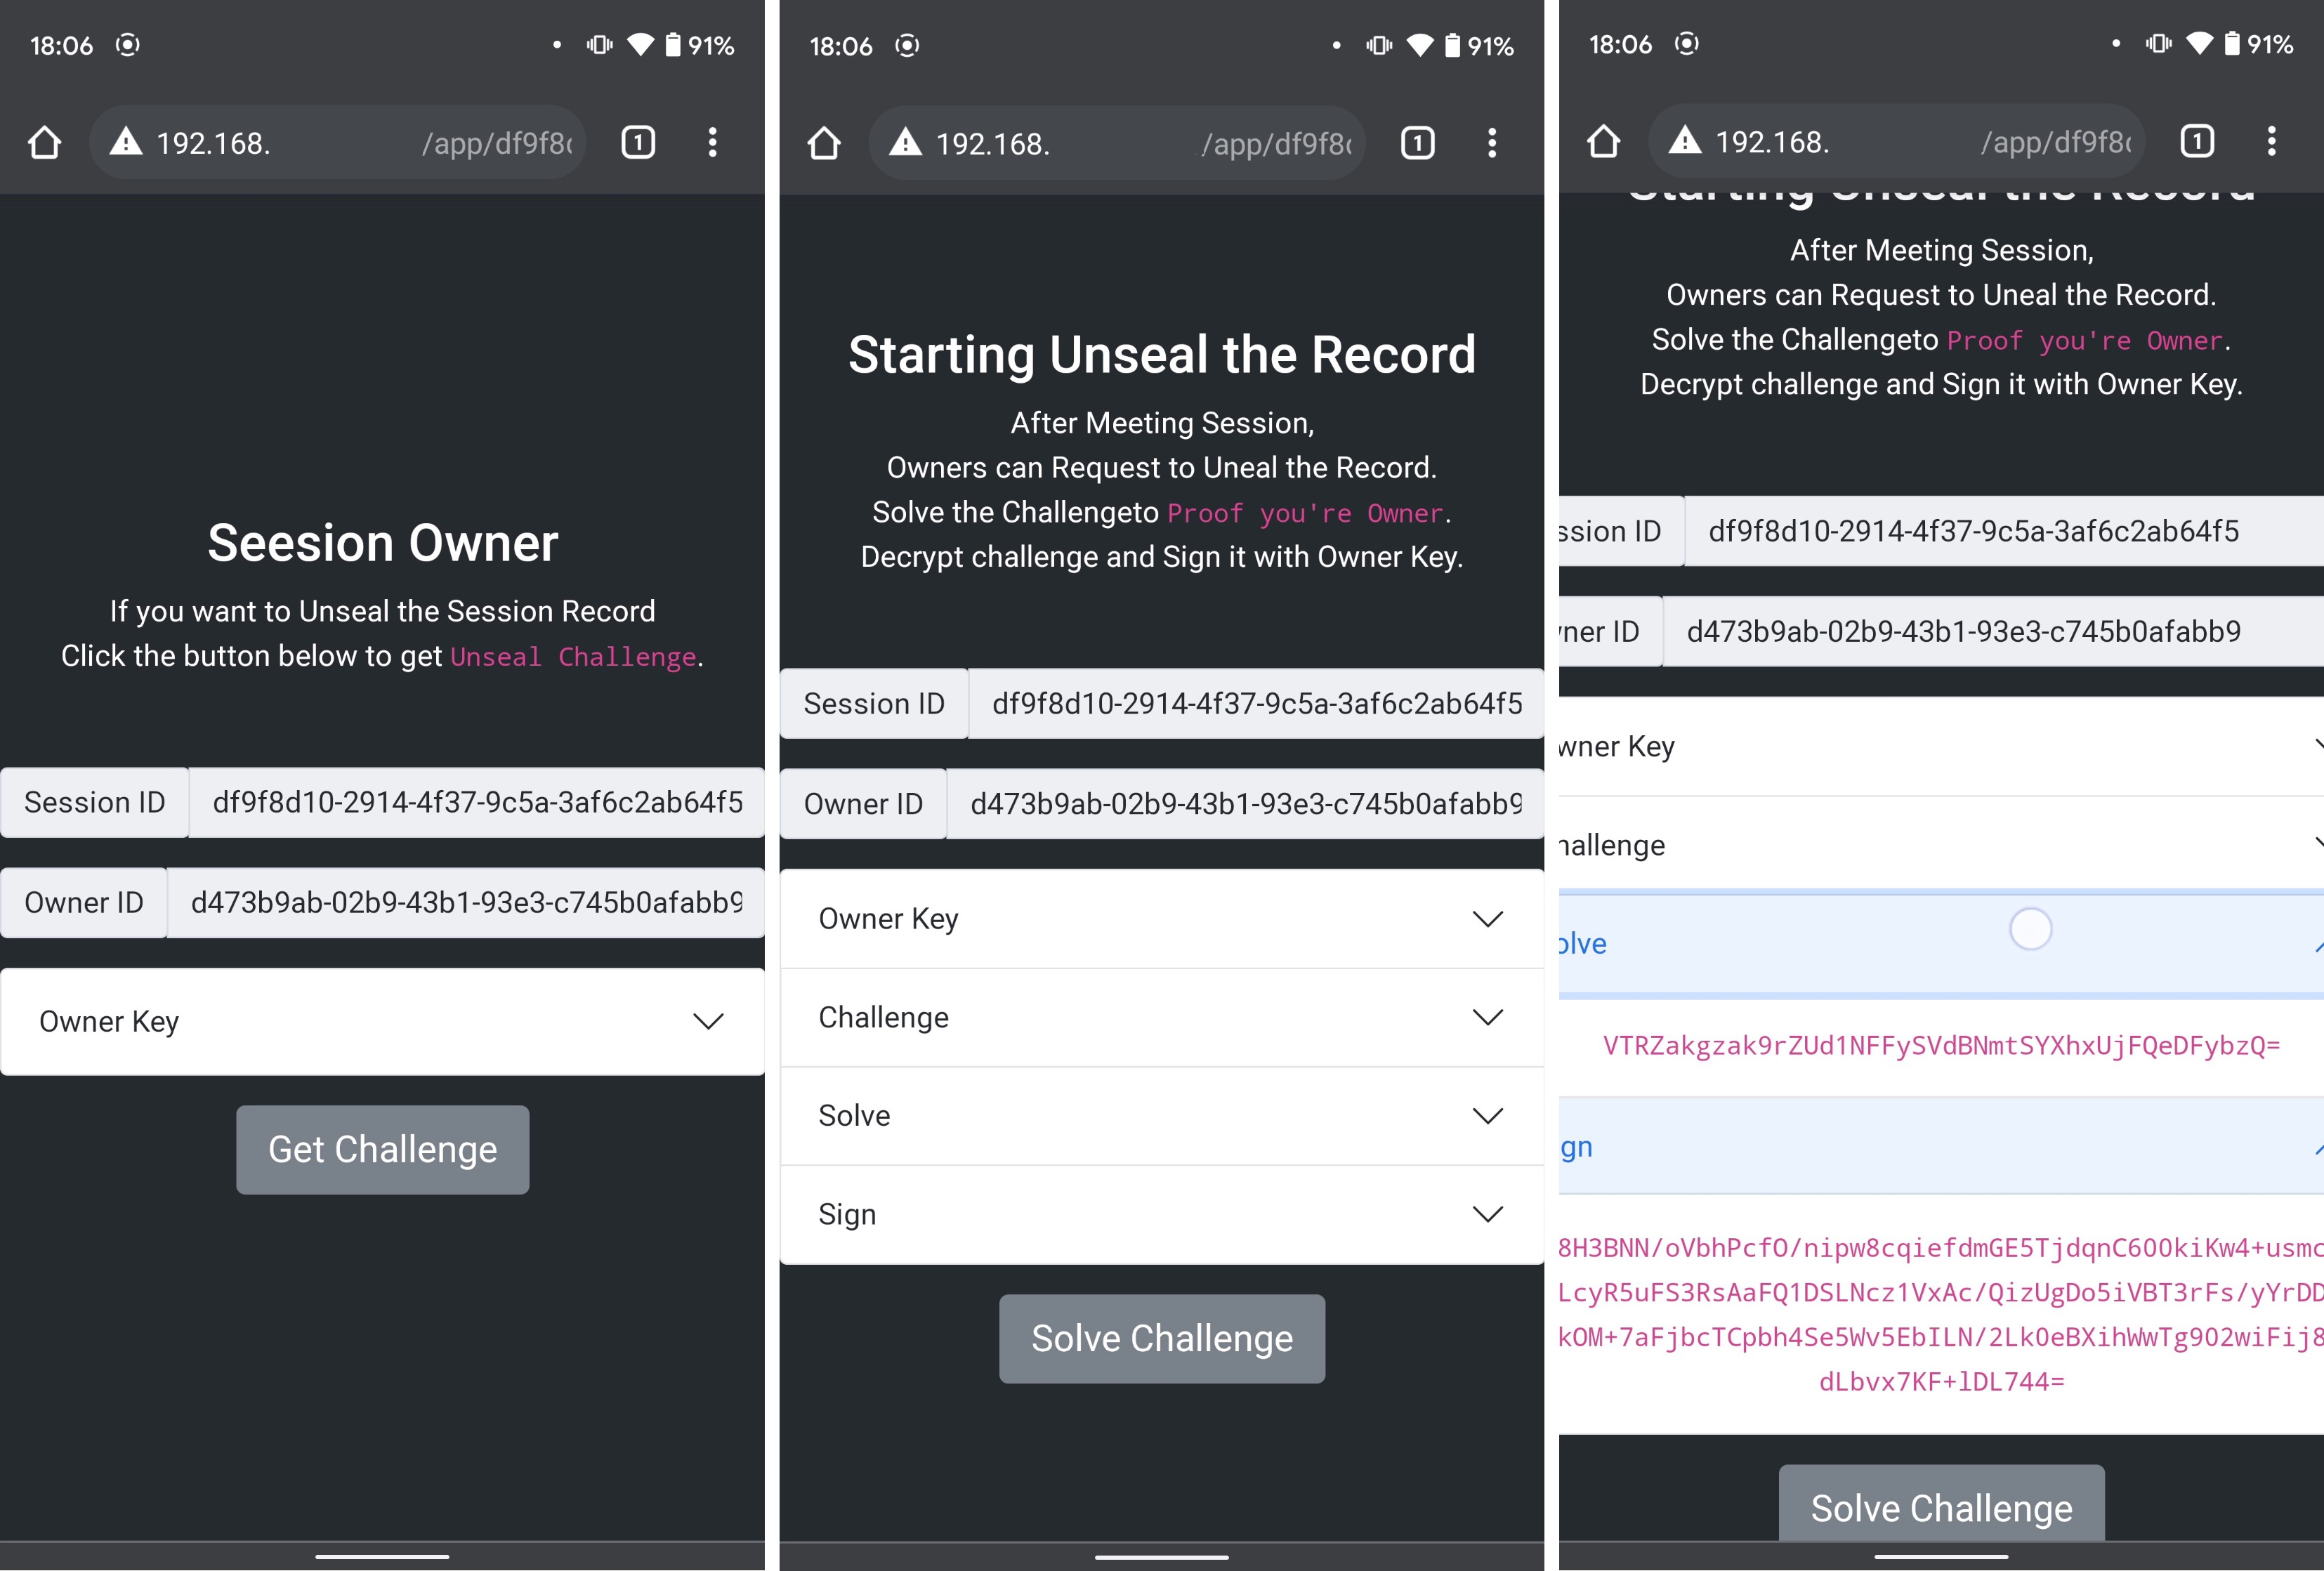
\includegraphics[width=0.75\textwidth]{app-2}
    \caption{行動應用程式會談主持者授權解封伺服器使用者介面}\label{fig:app-2}
\end{figure}

    在會談主持者成功授權解封伺服器 \DEFserver 後,向解封伺服器發起請求取得有效之會談聲音記錄。
如圖 \ref{fig:app-3} \nameref{fig:app-3}(右一)。

    此時封伺服器將受加密保護的純噪音之聲音記錄解密,
與含有噪音的受干擾會談聲音記錄透過聲音樣本的離散時間誤差推估函數與自適應噪音消除,還原獲得有效的會談聲音記錄。
執行過程中,如圖 \ref{fig:app-3} \nameref{fig:app-3}的(中)。
執行完成後,最終使會談主持者取得此有效之會談聲音記錄。
如圖 \ref{fig:app-3} \nameref{fig:app-3}(右一)。

\begin{figure}[H]
    \centering
    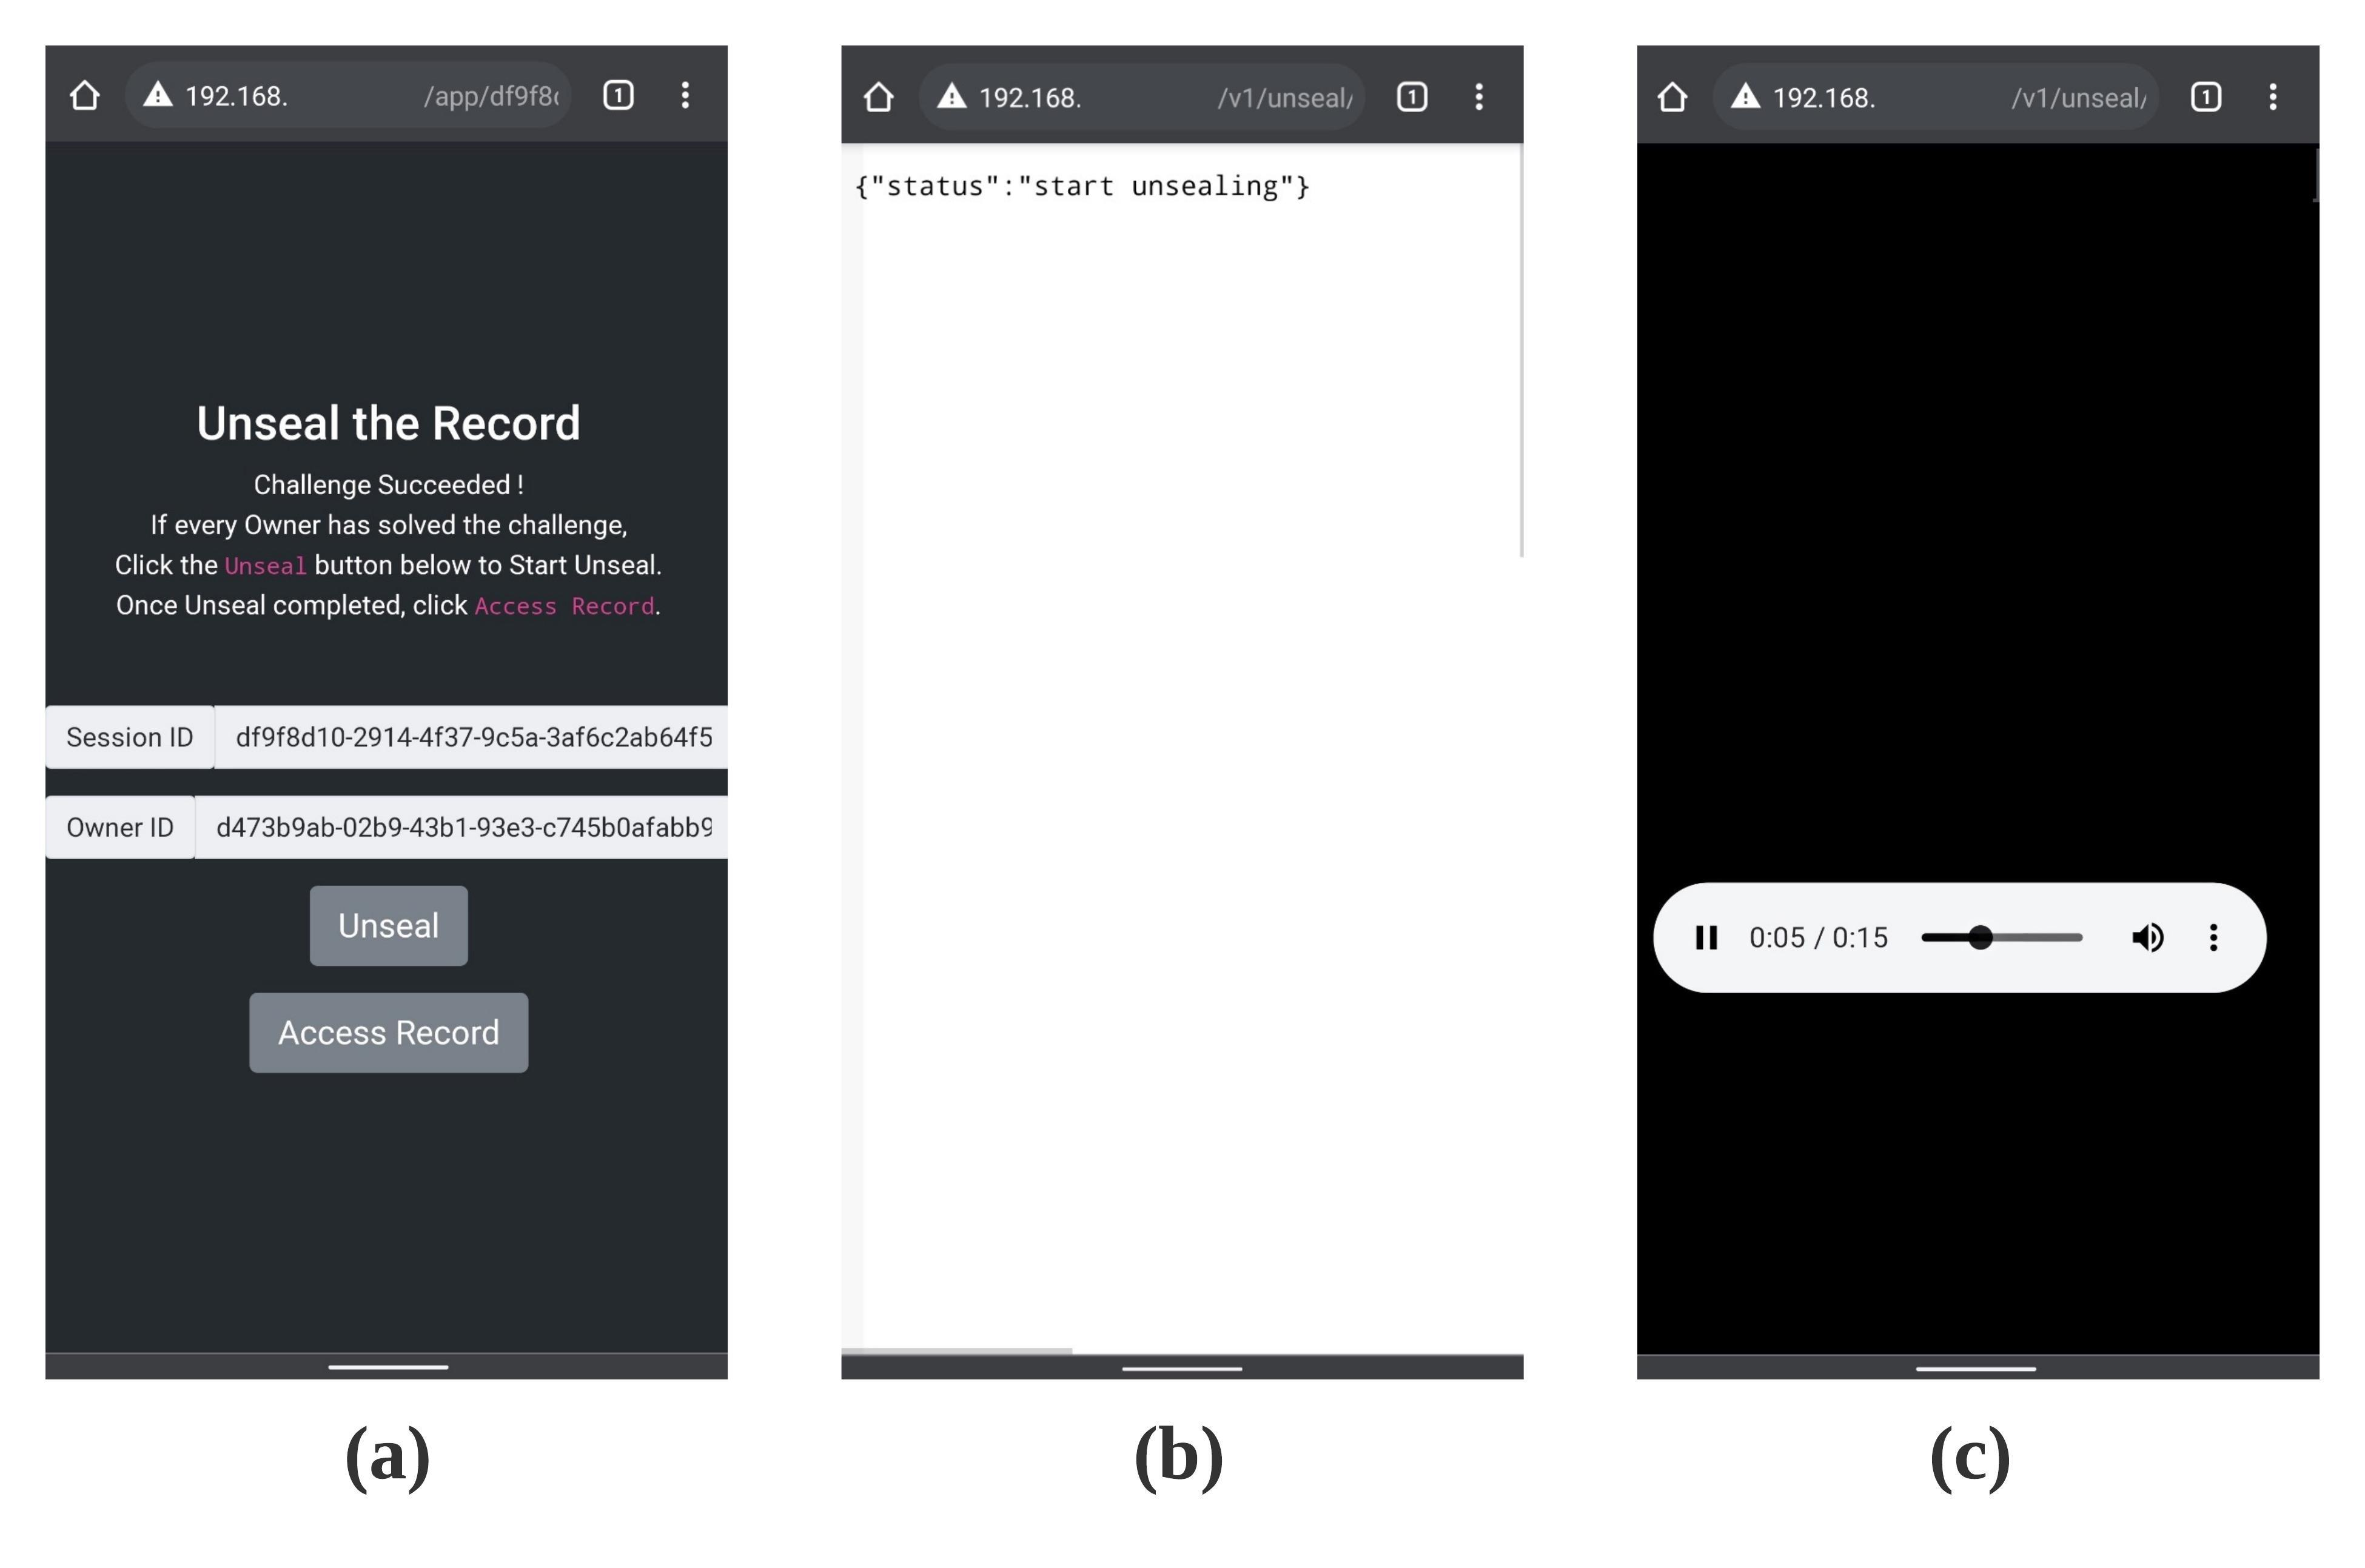
\includegraphics[width=0.75\textwidth]{app-3}
    \caption{行動應用程式取得會談聲音記錄使用者介面}\label{fig:app-3}
\end{figure}


\section{系統實驗}

\subsection{超音波麥克風干擾器之干擾效果分析}\label{subsec:exp-jammer}

    會談終端於會談進行間開啟超音波麥克風干擾器,因此鄰近的麥克風或周邊的聲音記錄裝置,
都將因受到其干擾而失效,場域內的會談參與者無法自行有效記錄會談的聲音內容。
此實驗音目的評估超聲波麥克風干擾器產生的干擾噪與音會談聲,
兩者在不同的信噪比下,超聲波麥克風干擾器的干擾效果。

    此實驗原理\cite{chen2019understanding}

    實驗儀器使用系統實作 \ref{subsec:impl-mbox} \nameref{subsec:impl-mbox}的超音波麥克風干擾器與錄音克風,
用於產生干擾噪音與錄音。搭配一 IEC 61672-1 標準 Class 2 等級的噪音計 TES-1350A,用於量測聲音分貝值。
實驗環境為背景噪音低於 40 dB的安靜室內空間。

    實驗步驟

    實驗結果
包含人耳聽感,與語音識別。


\subsection{主動式噪音消除效果分析}

    會談聲音與麥克風干擾器產生的干擾之信噪比下,噪音消除效果分析。
包含人耳聽感,與語音識別。

    實驗目的

    實驗原理

    實驗環境為使用前節 \ref{subsec:exp-jammer} \nameref{subsec:exp-jammer} 所產生的
純噪音聲音紀錄 \DEFrecN,與與欲消去噪音的會談聲音紀錄 \DEFrecJ,於噪音音量與會談內容不同的組合。

    實驗步驟

    實驗結果


\subsection{聲音樣本離散時間推估演算法}

    為提升噪音消除的成效,本研究提出聲音樣本離散時間推估演算法
透過將輸入噪音聲音紀錄 \DEFrecN 的離散時間索引值 \DEFpause 加上離散時間誤差值 \DEFshift,
來對齊修正噪音聲音紀錄 \DEFrecN 與欲消去噪音聲音紀錄 \DEFrecJ 的離散時間誤差。
由於純噪音聲音紀錄 \DEFrecN 與受干擾的會談聲音紀錄 \DEFrecJ 中的欲消去噪音,
在時域上波形有著高度關聯性,因此當兩聲音干涉抵銷後的能量會大幅度衰減。
如上所述,本研究提出透過累計整個離散時間序列每個樣本相減(兩聲音干涉抵銷)後總能量差的大小,作為是否對齊的參考指標。

    實驗目的一為驗證此對齊參考點 \DEFshift,其干涉抵銷後總能量差為最小值,且於離散時間序列上波形對齊。
目的二為觀察動態估計樣本標準差與平均數在執行過程中數值的變化,評估演算法終止條件是否符合預期,
解決歷遍所有可能 \DEFcandiSFT 累計能量差的時間複雜度膨脹快速問題。
原理如 \ref{subsec:exp-jammer} \nameref{subsec:exp-jammer}所述。

    實驗環境為準備一純噪音聲音紀錄 \DEFrecN,與與欲消去噪音的會談聲音紀錄 \DEFrecJ。
並實時輸出聲音樣本離散時間推估演算法執行時本標準差與平均數的數值並記錄。
實驗步驟如下:首先觀察兩樣本於離散時間上的波形前後誤差;接著執行此演算法得知離散時間誤差值 \DEFshift;
接著觀察離散時間索引值 \DEFpause 加上離散時間誤差值 \DEFshift 後兩樣本於離散時間上的波形前後誤差;
最後分析各項數值於執行過程中數值的變化。

    實驗結果如下:

\begin{figure}[H]
    \centering
    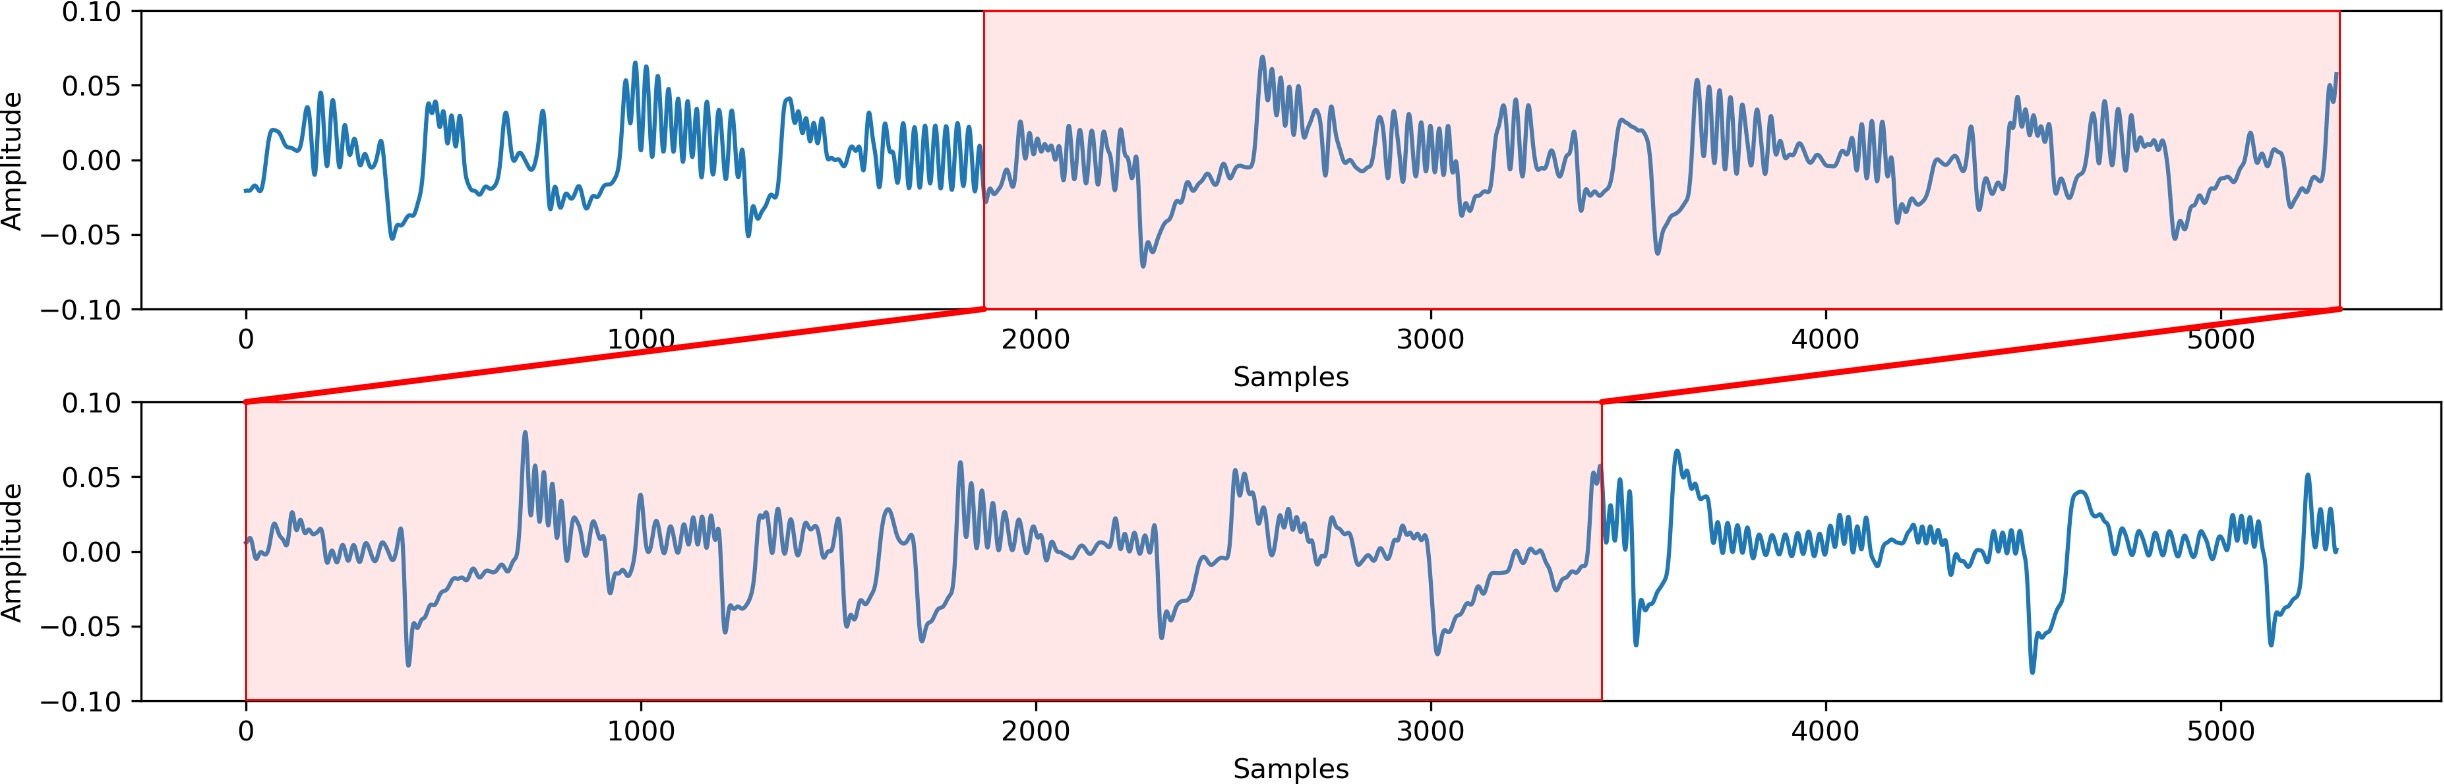
\includegraphics[width=0.95\textwidth]{exp-shift-1}
    \caption{聲音樣本對齊前波形圖}\label{fig:exp-shift-1}
\end{figure}

\begin{figure}[H]
    \centering
    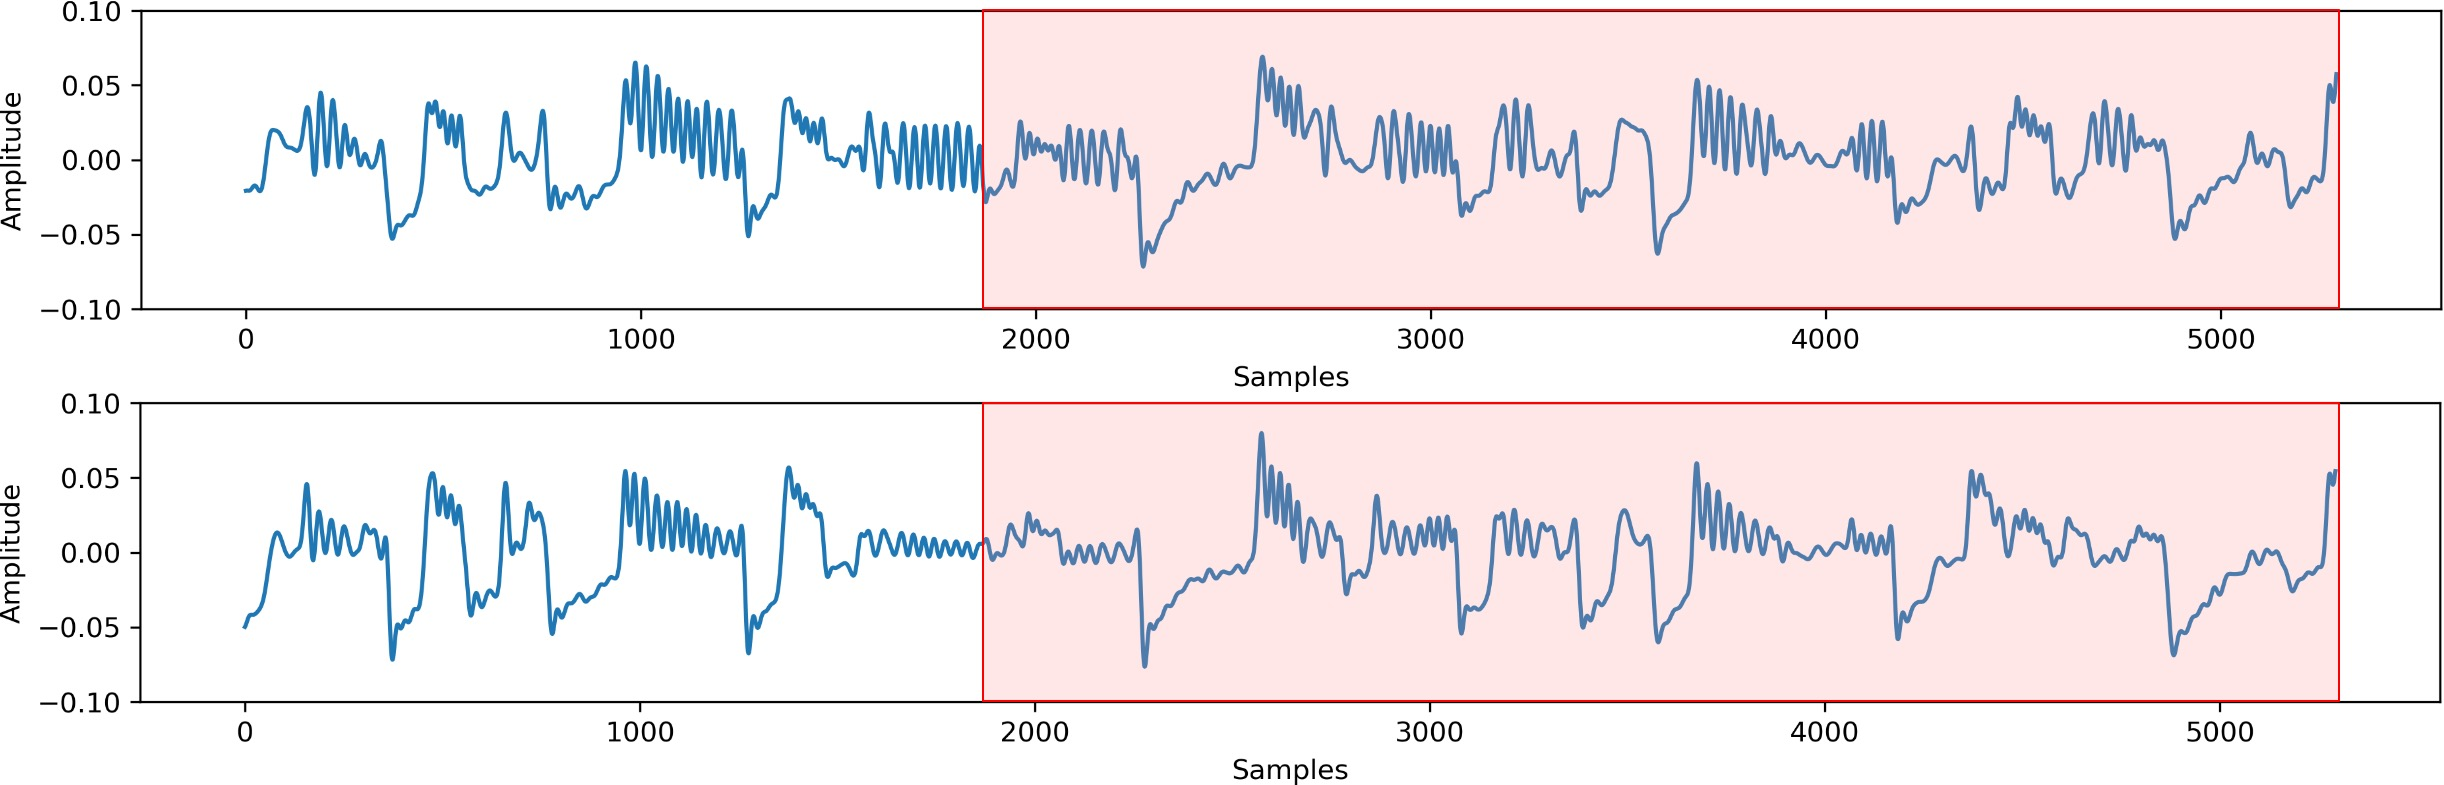
\includegraphics[width=0.95\textwidth]{exp-shift-2}
    \caption{聲音樣本對齊後波形圖}\label{fig:exp-shift-2}
\end{figure}

\begin{figure}[H]
    \centering
    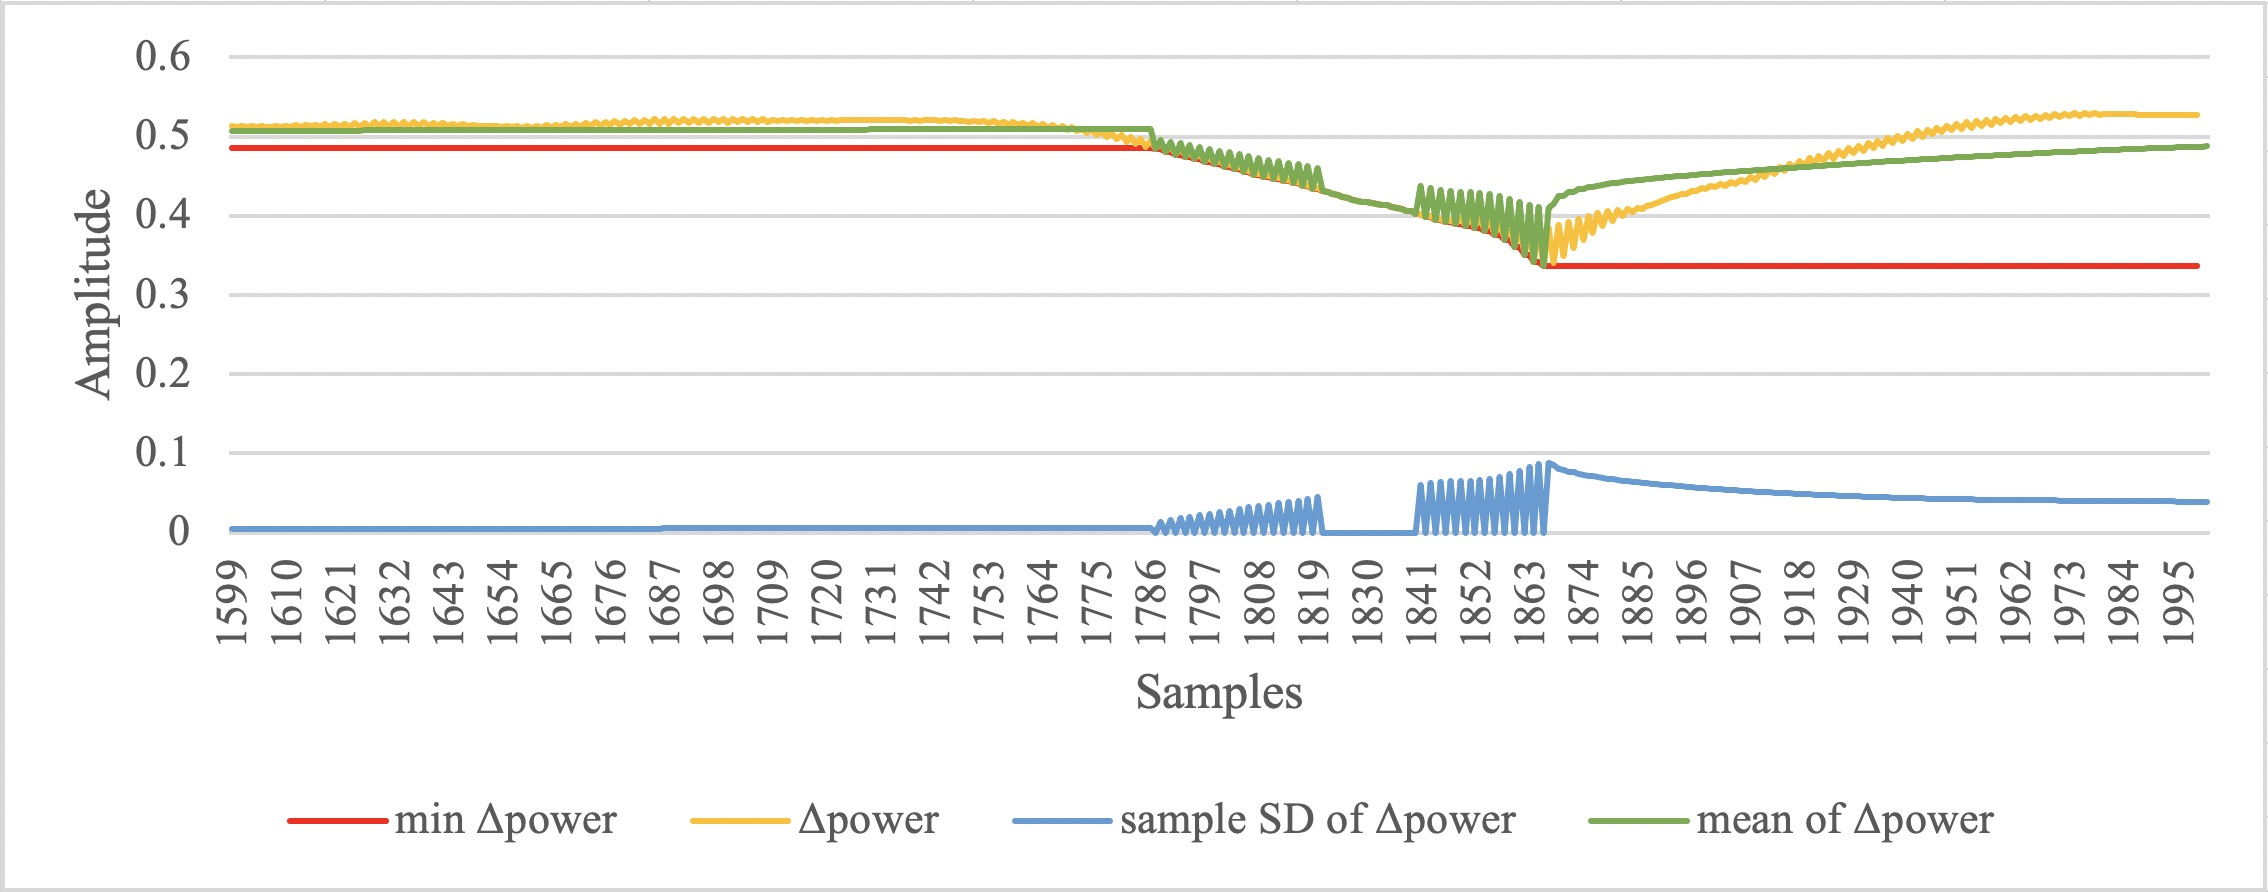
\includegraphics[width=0.95\textwidth]{exp-shift-3}
    \caption{聲音樣本離散時間推估演算法執行時數值圖}\label{fig:exp-shift-3}
\end{figure}

\begin{figure}[H]
    \centering
    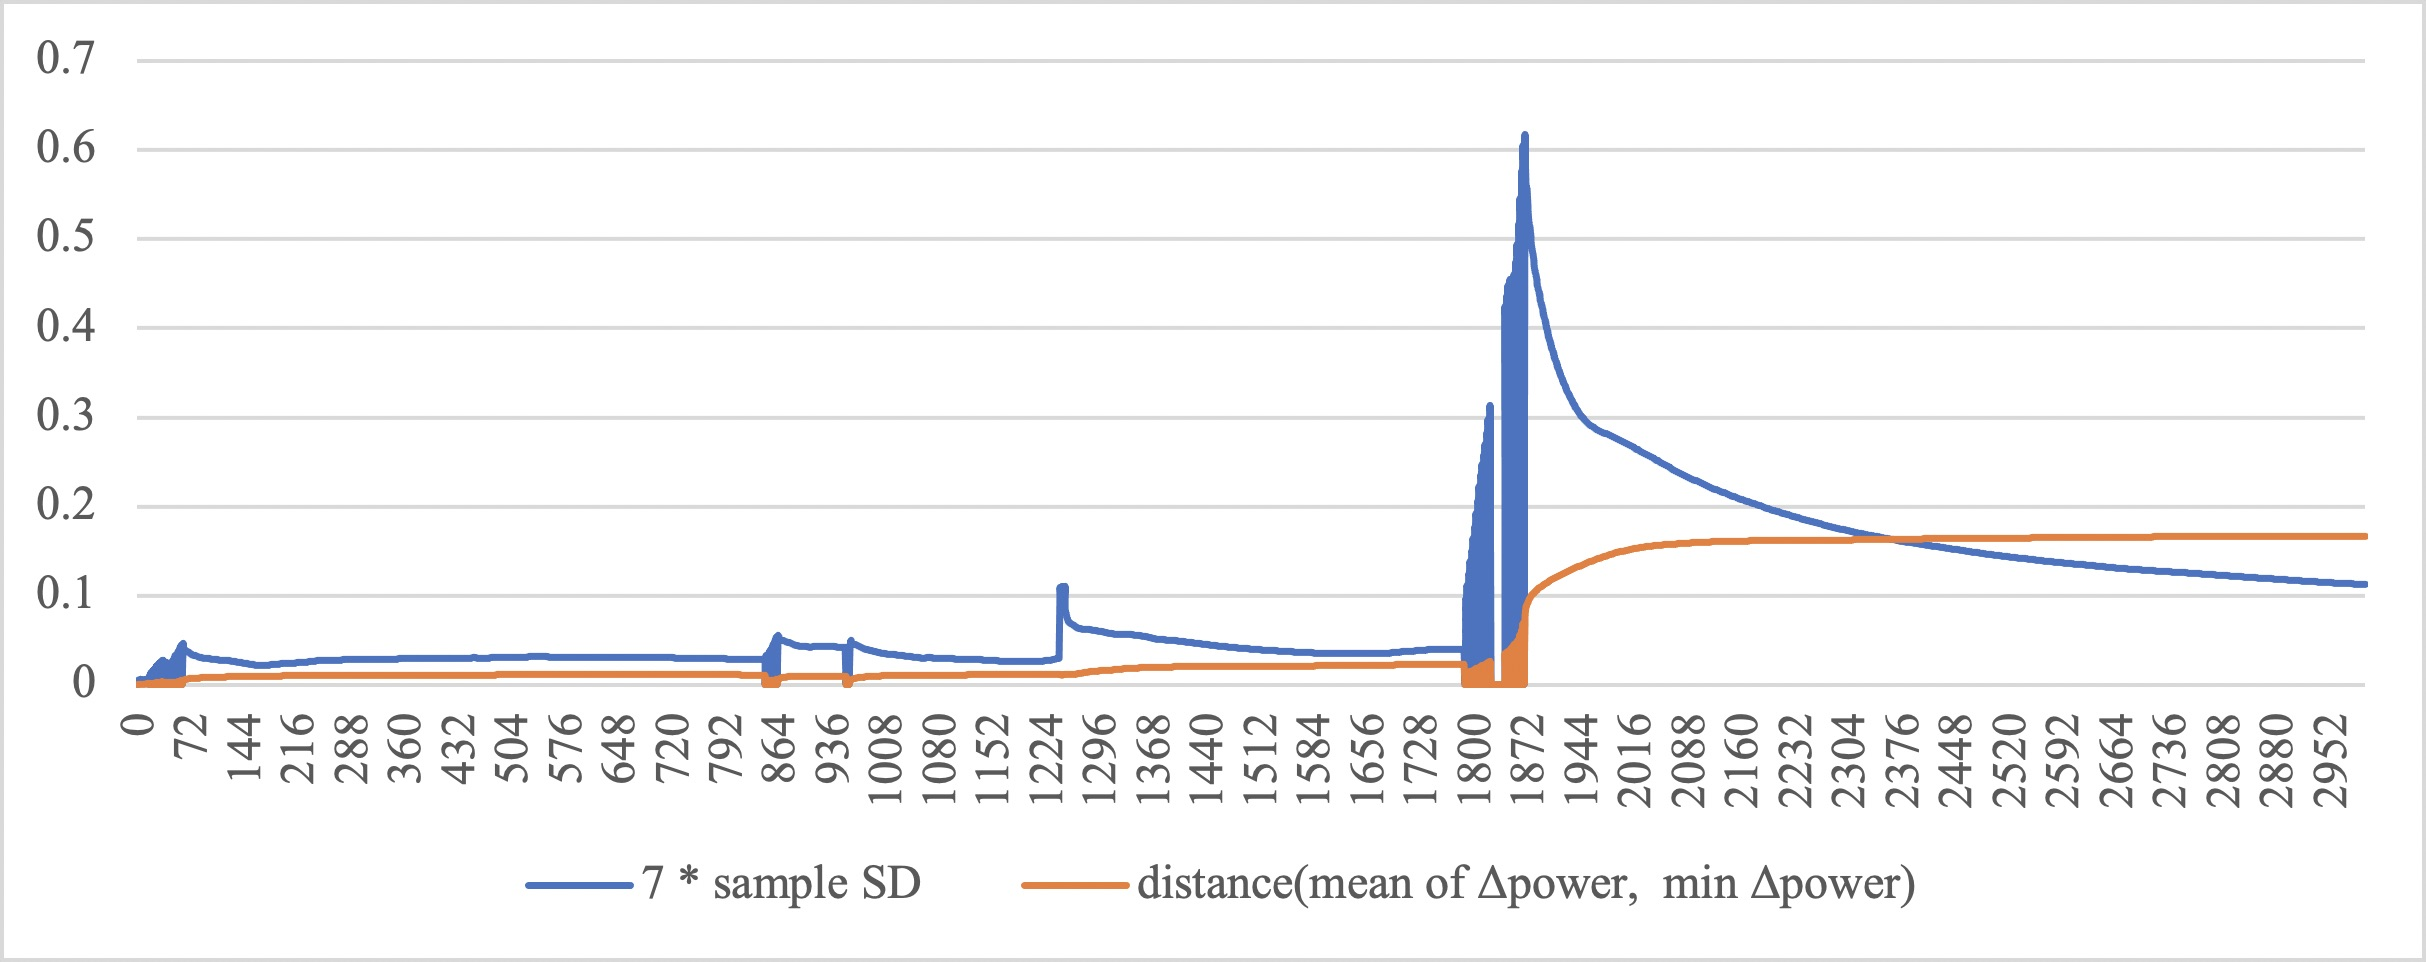
\includegraphics[width=0.95\textwidth]{exp-shift-4}
    \caption{最小累積能量差與七倍標準差變化圖}\label{fig:exp-shift-4}
\end{figure}


\subsection{解封會談聲音記錄分析性能分析}

    伺服器獲得授權後,執行聲音樣本離散時間推估演算法與主動式噪音消除來還原產生有效的會談聲音紀錄,
其錄音長度與執行時間的時間複雜度性能分析。

    實驗目的

    實驗原理

    實驗儀器
    實驗環境

    實驗步驟

    實驗結果


\section{實驗結果與討論}

    本研究所設計之系統可以確保 Server 在 Running {\it Meeting Session}結束後,
直到成功解封 ({\it Unseal})之前,\DEFrecREV 保有機密性。

\begin{figure}[H]
    \centering
    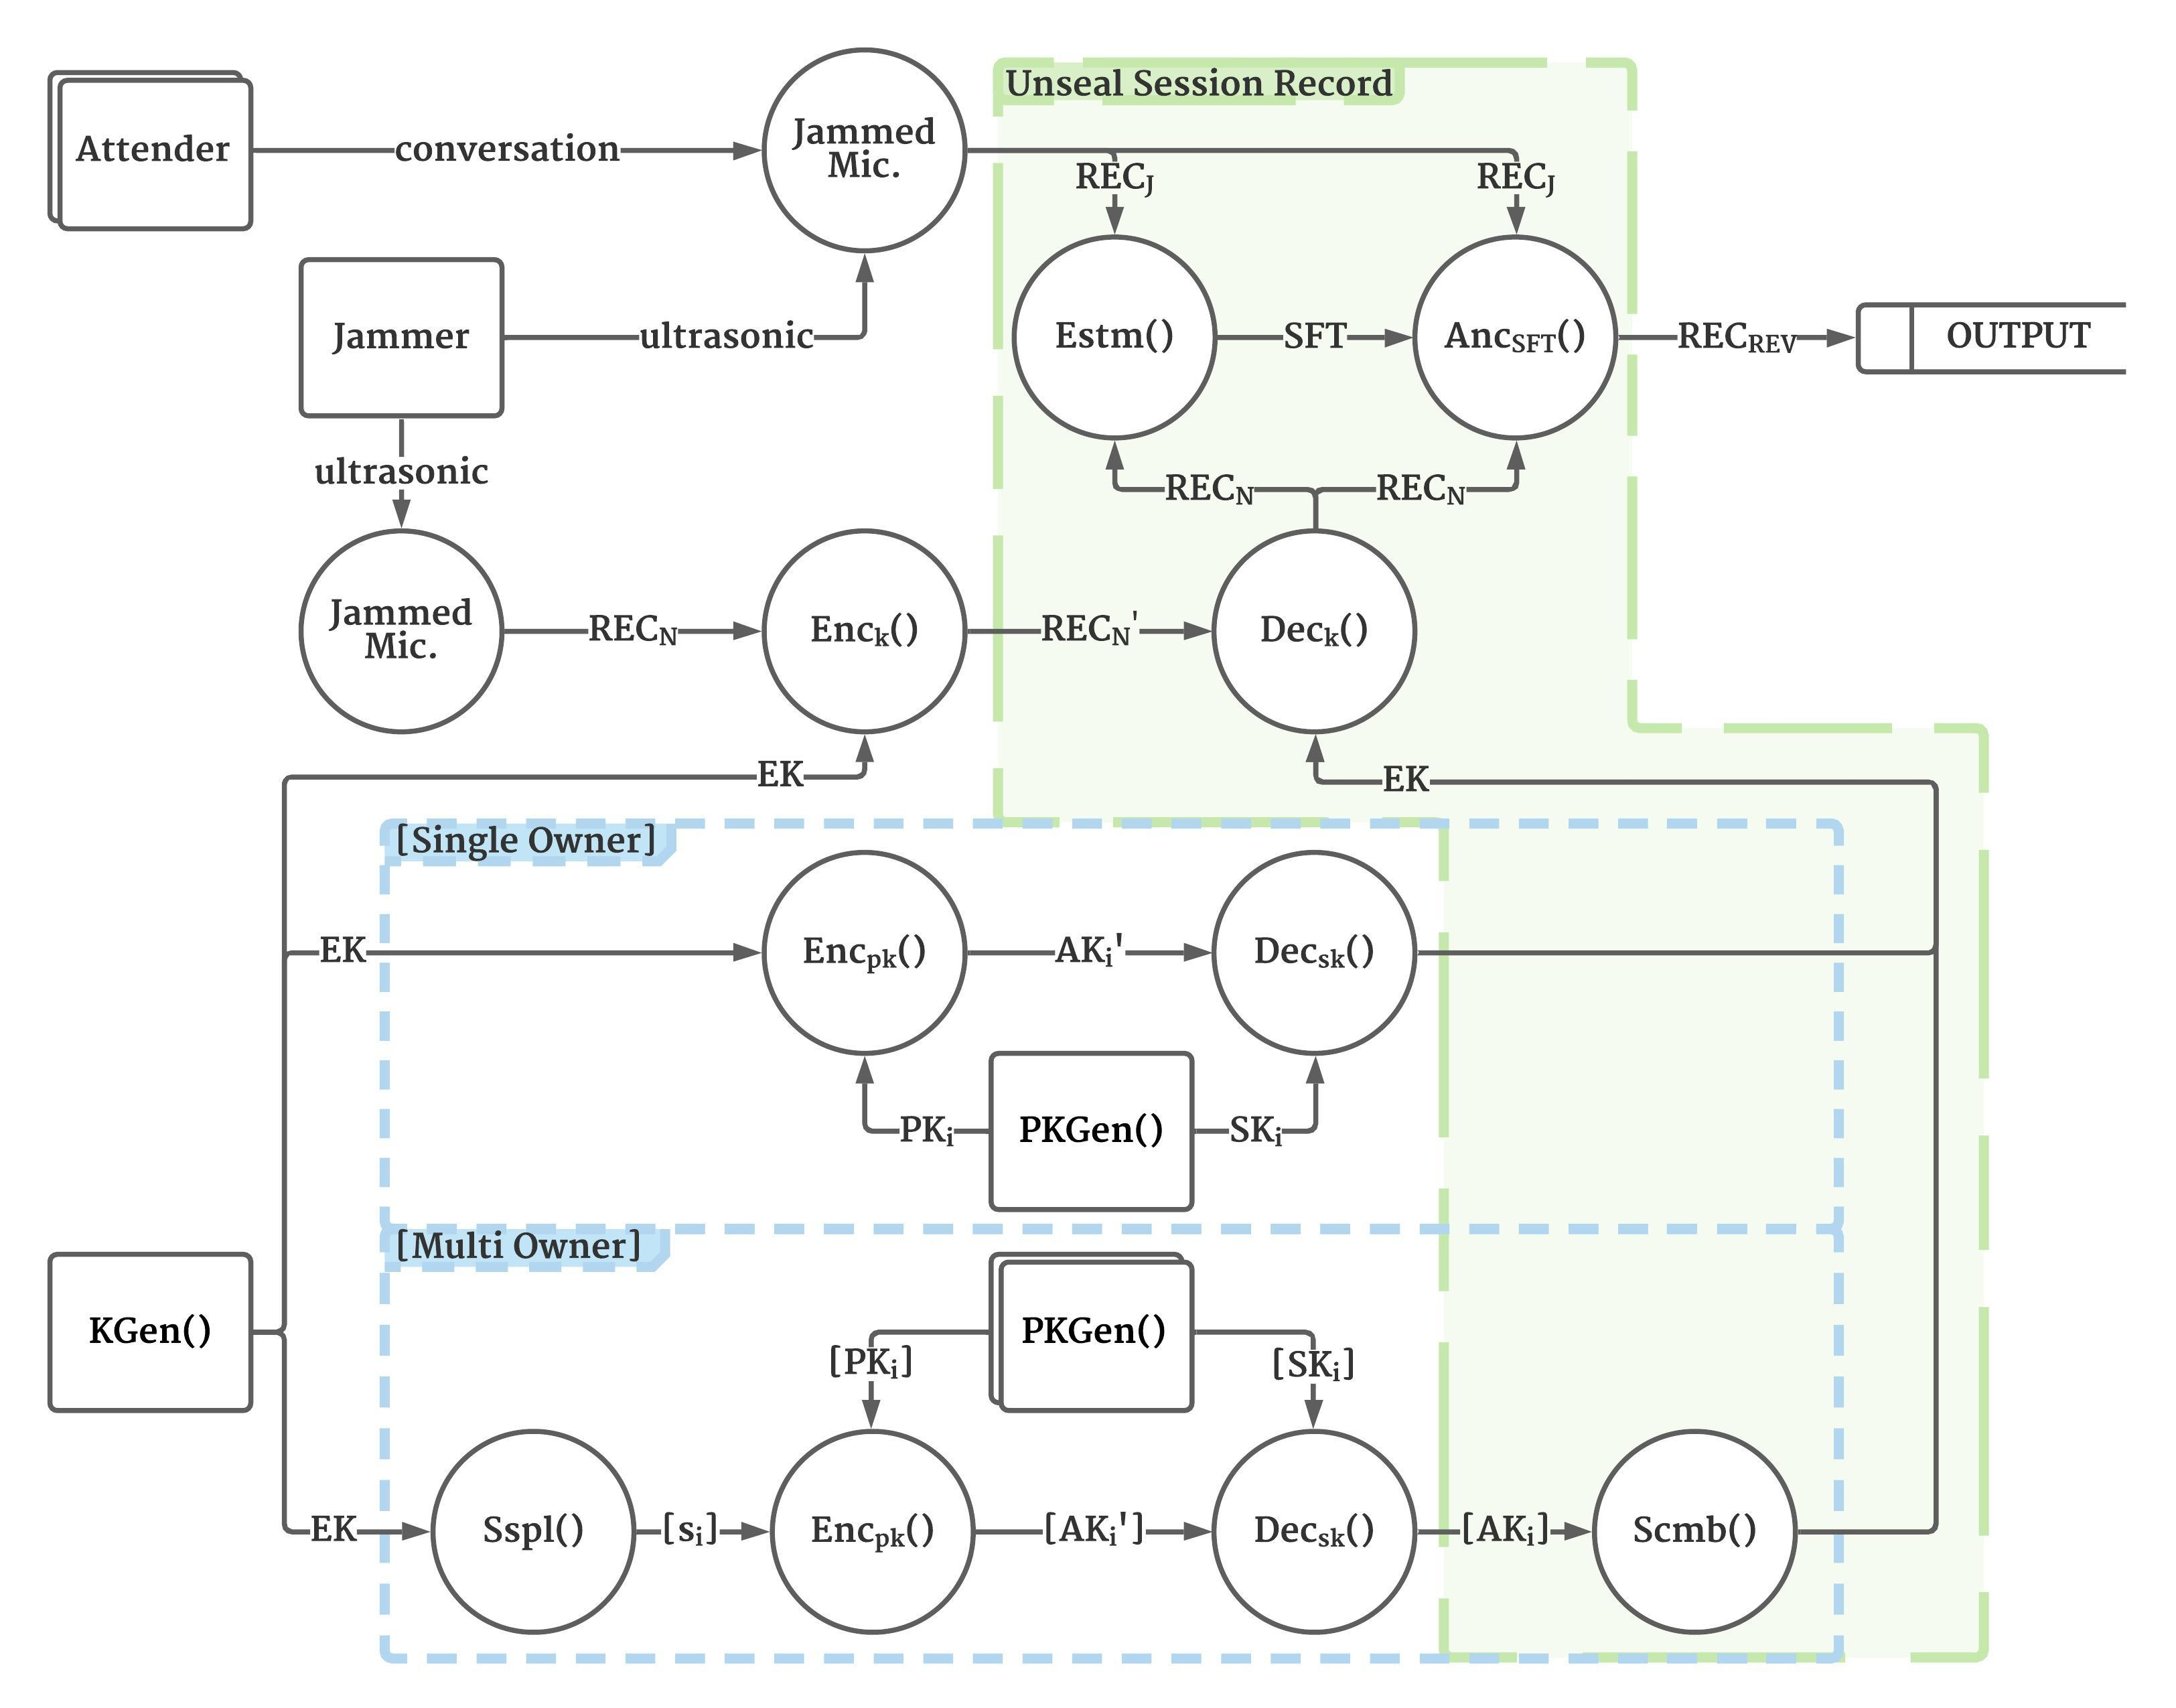
\includegraphics[width=1.0\textwidth]{system-data-flow}
    \caption{系統資料流程圖}\label{fig:system-data-flow}
\end{figure}